\subsection{K-Nearest-Neighbor} \label{ssec:knn}
Der \textit{K-Nearest-Neighbor (KNN)}, zu Deutsch 'K-nächste Nachbarn', ist ein Machine Learning Algorithmus, der 1951 von Joseph Hodeges und Evelyn Fix entwickelt und später von Thomas Cover weiterentwickelt wurde.\\\hfill
Der \acp{KNN} eignet sich zur Klassifizierung und Regression von Objekten, wurde im Laufe dieser Arbeit aber ausschließlich zur Klassifizierung verwendet. Der Algorithmus gehört zu den überwachten Lernverfahren, d.h. er nutzt als Eingabeobjekte während des Trainings ein Bild, das später auch zur Klassifizierung übergeben wird. Zusätzlich wird auch noch ein Label mit jedem Bild übergeben, das angibt, um welches Objekt es sich handelt. \\\hfill
Da der \textit{KNN-Algorithmus} zur Kategorie der \textit{Lazy Learner} gehört, erstellt dieser kein Modell während der Trainingsphase, sondern erst, sobald eine Klassifizierungsanfrage stattfindet. Während der Trainingsphase passen \textit{Lazy Learner} keine Gewichte an, um damit genauere Vorhersagen treffen zu können, sondern sie speichern lediglich die Trainingsdaten anhand ihrer Merkmale in einem $\mathcal{R}^N$ dimensionalem Diagramm ab, \textit{N} entspricht hierbei der Anzahl der Merkmale. Diese Merkmale bilden später die Grundlage für die Klassifizierung. Dieser Entscheidungsprozess ist dabei einer der denkbar einfachsten, denn es wird lediglich mit den \textit{k} nächsten Nachbarn eine Mehrheitsentscheidung getroffen. Das Ergebnis davon bestimmt die Kategorie des neuen Objektes.\par

Der Entscheidungsprozess des \textit{KNN} läuft dabei in 5 Schritten ab:
\begin{enumerate}
    \item Bestimmen von \textit{K}
    \item Berechnen der Distanz anderer Objekte
    \item \textit{K} nächste Nachbarn bestimmen
    \item Bestimmung der Kategorie der Nachbarn
    \item Kategorie zuweisen
\end{enumerate}

\subsubsection{1. Bestimmen von \textit{K}}
\textit{K} ist eine feste Konstante, die vom Benutzer festgelegt wird. Dabei gibt es keinen festen Wert, um die perfekte Anzahl an Nachbarn zu bestimmen. Je nach Einsatzzweck kann es sinnvoll sein, ein höheres oder niedrigeres \textit{k} zu wählen. Bei einer binären Klassifizierung, also nur zwei zu bestimmende Klassen, ist es sinnvoll ein ungerades \textit{k} zu wählen. Dadurch kann es später bei der Mehrheitsentscheidung nicht zu einem Unentschieden kommen. Wenn es nur darum geht den nächsten Nachbarn zu bestimmen, also \textit{k} = 1 ist, nennt man dies den \textit{Nearest Neighbor} oder auch \textit{1-Nearest Neighbor}.\\\hfill
Der Schritt zur Bestimmung der Konstante \textit{k} wird dabei nur beim Erstellen des Algorithmus durchgeführt und danach diesem permanent übergeben.

\subsubsection{2. Berechnen der Distanz anderer Objekte}
Wird dem Algorithmus nach der Trainingsphase ein neues Objekt übergeben, wird es anhand seiner Merkmale in das Diagramm, das zuvor erstellte wurde, eingetragen. Von dem neu eingetragenen Objekt wird nun die Distanz zu allen anderen gespeicherten Objekten bestimmt. Zur Bestimmung dieses Abstandes können dabei verschiedene Verfahren angewendet werden. Die Populärsten sind dabei \textit{Euklidischer Distanz} / \textit{Abstand} und die \textit{Manhattan-Metrik} oder auch \textit{Mannheimer Metrik} genannt.\par

Die \textit{Euklidische Distanz} ist die Luftlinie zwischen zwei Punkten und gibt damit die direkte Distanz wieder. Sie wird wie folgt berechnet:
\[\sqrt{\sum_{i=0}^n(x_i - y_i)^2}\]
$n$ ist dabei die Anzahl der Merkmale, die jedes Objekt besitzt.\\\hfill
$x$ \& $y$ sind die Position der beiden Objekte.\par

Die \textit{Manhattan-Metrik} bestimmt die Distanz anhand der Summe der absoluten Differenz der einzelnen Koordinaten.
\[\sum_{i=0}^n|x_i - y_i|\]
$n$ entspricht auch hier wieder der Anzahl der Merkmale.\\\hfill
$x$ \& $y$ entsprechen ebenso wieder den Koordinaten zweier Objekte.

\subsubsection{3. \textit{k} nächste Nachbarn bestimmen}
Mithilfe der Distanz können wir nun feststellen welche die nächsten Nachbarn zu unserem neuen Objekt sind. Dabei sind nur die \textit{k}-nächsten von Interesse.

\subsubsection{4. Bestimmung der Kategorie der Nachbarn}
Im vierten Schritt stellen wir fest, zu welcher Kategorie jeder der \textit{k} Nachbarn gehört und zählen diese. Bei anderen Varianten des \textit{KNN} werden auch je nach Entfernung zum neuen Objekt Gewichtungen verteilt, dadurch erhält der nächste Punkt die höchste Gewichtung und je weiter entfernt, desto geringer das Gewicht. Hierdurch wird mehr auf räumliche Nähe zu einzelnen Punkten geachtet und weniger zu großen Ansammlungen.

\subsubsection{5. Kategorie zuweisen}
Als Letztes müssen wir dem neuen Punkt eine Kategorie zuweisen. Dabei wird die am häufigsten unter den Nachbarn vertretende Kategorie gewählt. Bei der gewichteten Variante wird die Kategorie mit dem größten Gewicht gewählt.\cite{script_korn}\par

\begin{figure}[H]
    \centering
    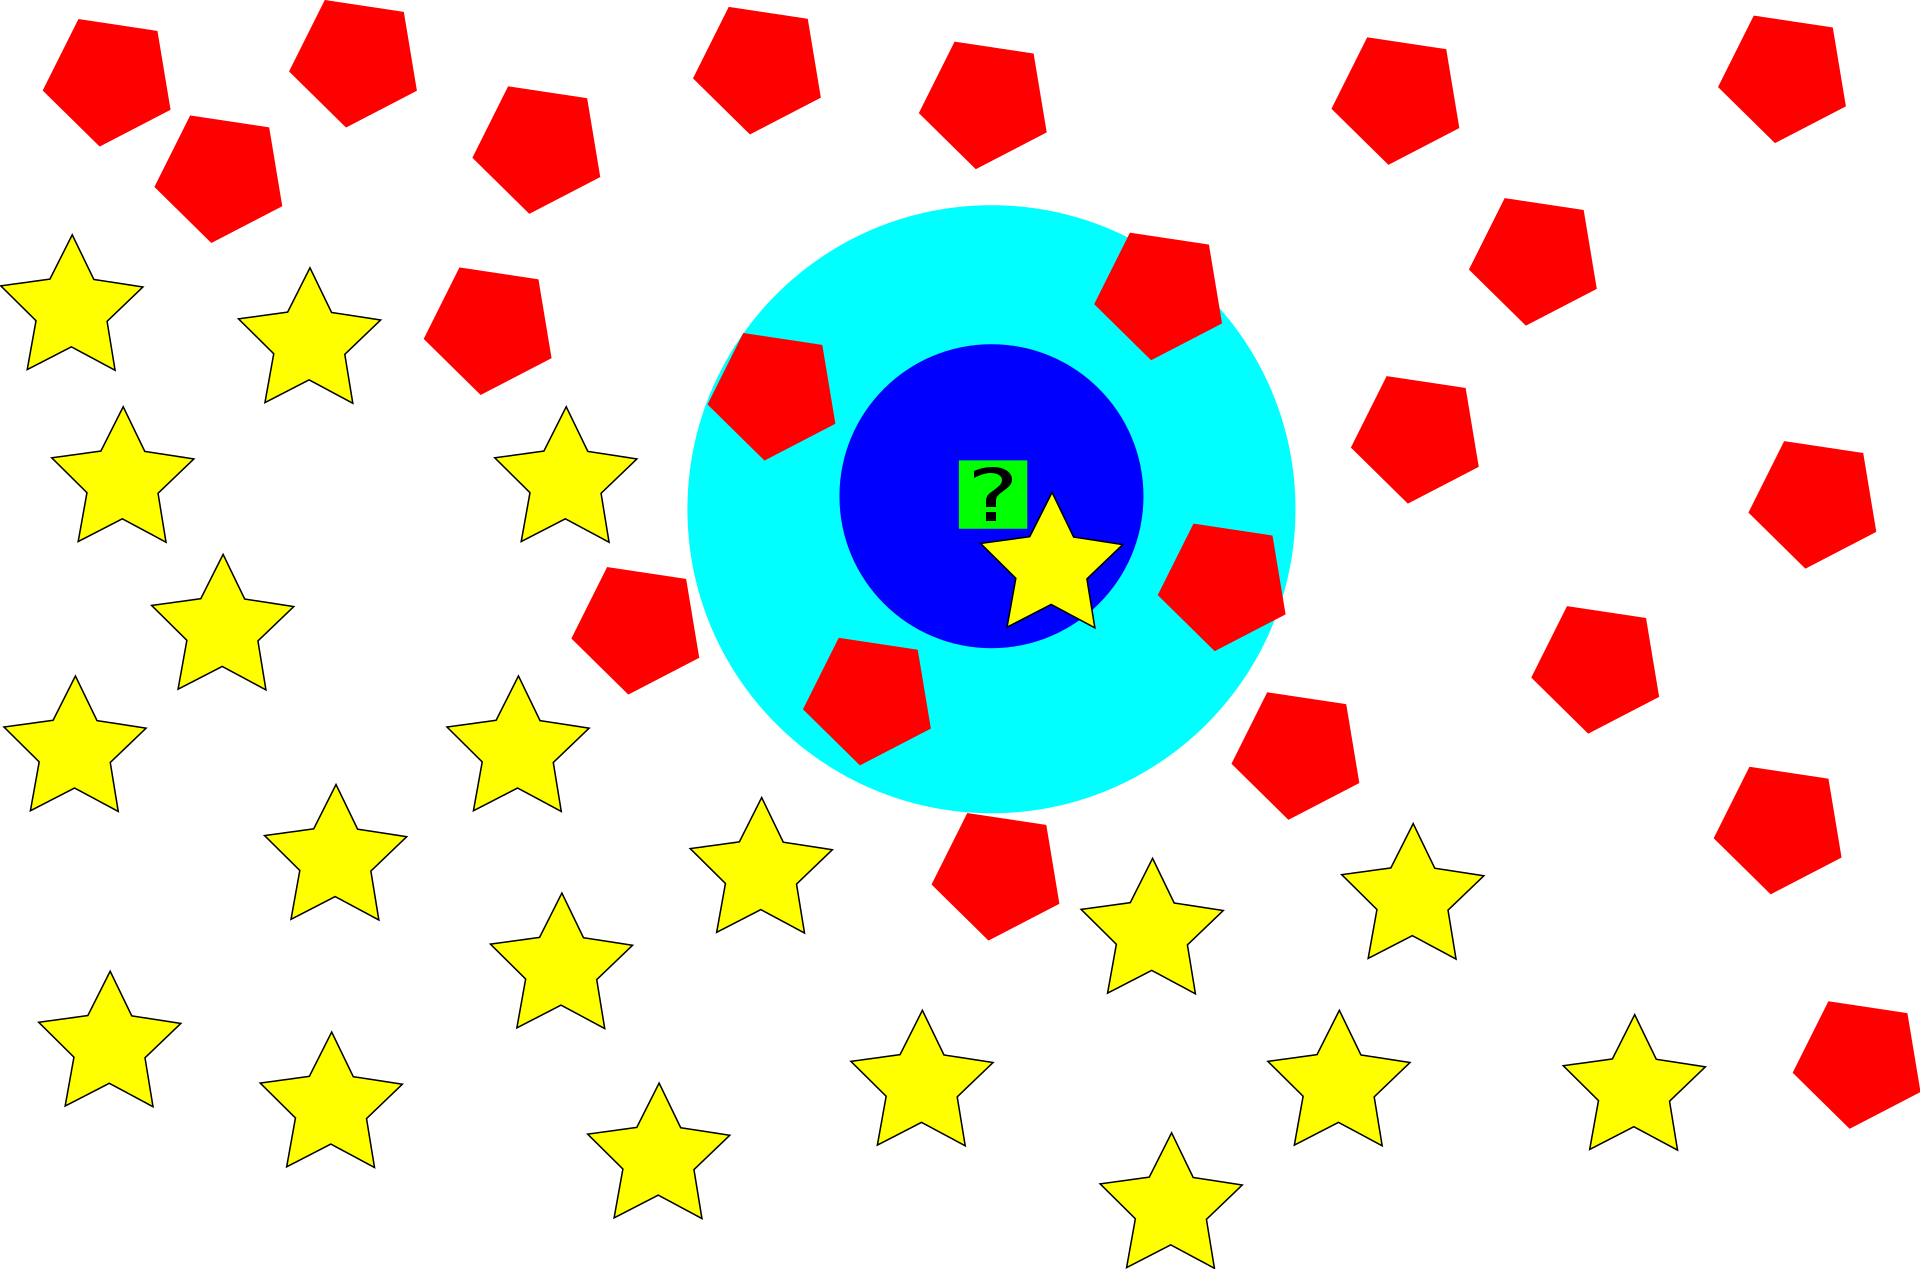
\includegraphics[width=\imgMed]{images/theory/knn.png}
    \caption{Funktionsweise des \textit{KNN}}
    \label{fig:knn_function}
\end{figure}

Die Grafik \ref{fig:knn_function} demonstriert den Entscheidungsprozess des \textit{KNN}. Es werden immer nur die \textit{k} nächsten Nachbarn beachtet. So wird das neue Objekt bei \textit{k} = 1 der Kategorie \textit{gelber Stern} zugeordnet, dargestellt durch den dunkelblauen Kreis. Beachtet man hingegen die fünf nächsten Nachbarn, also hat \textit{k} = 5, hat man \textit{1x gelber Stern} und \textit{4x rotes Fünfeck}, dargestellt durch den hellblauen Kreis. Durch die Mehrheitsentscheidung wird das neue Objekt nun der Kategorie \textit{rotes Fünfeck} zugeteilt.

\subsubsection{Bewertung des \textit{K-Nearest-Neighbor}}
Der \textit{KNN} wird wie die beiden anderen Algorithmen nach den Kriterien Komplexität, Genauigkeit, Präzision und Einfachheit der Umsetzung bewertet.\\\hfill
Da der \textit{KNN} während des Trainings lediglich Daten speichert, besitzt er hierbei keine Komplexität. Beim Klassifizierern von Testdaten beträgt seine Komplexität $O(np)$, $n$ entspricht dabei der Anzahl von Testdaten und $p$ die Anzahl der Features.\cite{complexity} \par
Die drei Punkte Genauigkeit, Präzision und Einfachheit der Umsetzung können mit einem kurzen Testprogramm bewertet werden, das in \ref{lst:test_knn} zu sehen ist. Hierfür gibt es in der Programmiersprache \textbf{Python} die Bibliothek \textbf{Scikit-learn}. Diese neben \textit{KNN} noch einige weitere bereits fertig implementierte Machine Learning Algorithmen. Außerdem bietet sie Zugang zu verschiedenen Datensätzen, dazu gehört auch der \textbf{MNIST}-Datensatz. \\\hfill
Im Programm werden nun zunächst einmal die benötigten Funktionen und Klassen aus den verschiedenen Abhängigkeiten importiert. Anschließend werden die Daten vorbereitet. Dafür wird der Datensatz geladen und für die bessere Verarbeitung in ein \textbf{NumPy}-Array gewandelt und danach in die Trainings- und Testdaten aufgeteilt. Der \textit{KNN} wird nun mit den Werten $k = 5$, $p = 2$ und der \textbf{minkowski-Metrik} initialisiert. Der Parameter $p$ gibt dabei die Power der Metrik an. So verhält sich die \textit{Minkowski-Metrik} für $p = 1$ wie die \textit{Manhattan-Metrik} und bei $p = 2$ wie die \textit{Euklidische Distanz}. Diesem \textit{KNN} werden jetzt die Trainingsdaten übergeben und anschließend wird er mit den Testdaten getestet. Zum Schluss werden noch einige Ausgaben erzeugt, um die benötigten Informationen zu erhalten.\\\hfill

\begin{minipage}{\textwidth}
    \begin{lstlisting}[language=Python, caption=Pythoncode zum Testen des KNN, label=lst:test_knn]
# Importieren der Abhaengigkeiten
from sklearn import metrics
from sklearn.datasets import load_digits
from sklearn.neighbors import KNeighborsClassifier
from sklearn.model_selection import train_test_split

# Vorbereiten des Datensatzes
digits = load_digits()
n_samples = len(digits.images)
data = digits.images.reshape((n_samples, -1))

# Aufteilen in Trainings- und Testdaten
X_train, X_test, y_train, y_test = train_test_split(
    data, digits.target, test_size=0.5, shuffle=False)

# Initialisieren des KNN
KNN_classifier = KNeighborsClassifier(
    n_neighbors=5, p=2, metric='minkowski')

# Trainingsdaten speichern
KNN_classifier.fit(X_train, y_train)

# Klassifizieren der Testdaten
predicted = KNN_classifier.predict(X_test)

# Ergebnisse ausgeben
report = metrics.classification_report(y_test, predicted)
print("\nKlassifizierungsbericht %s:\n%s\n" %
        (KNN_classifier, report))
score = KNN_classifier.score(X_test, y_test)
print("Genauigkeit des Algorithmus: ", score)
    \end{lstlisting}
\end{minipage}
Die Ausgabe des Programmes gibt damit sofort die Präzision und Genauigkeit \textit{KNN} an.\par
\begin{minipage}{\textwidth}
    \begin{lstlisting}[language=Bash, caption=Testergebnisse des KNN, label=lst:testergebnis_knn]
        Klassifizierungsbericht KNeighborsClassifier():
            precision    recall  f1-score   support

         0       0.99      1.00      0.99        88
         1       0.95      0.98      0.96        91
         2       0.98      0.93      0.95        86
         3       0.89      0.90      0.90        91
         4       1.00      0.95      0.97        92
         5       0.96      0.98      0.97        91
         6       0.99      1.00      0.99        91
         7       0.95      1.00      0.97        89
         8       0.95      0.90      0.92        88
         9       0.91      0.92      0.92        92

accuracy                               0.96       899
macro avg          0.96      0.96      0.96       899
weighted avg       0.96      0.96      0.96       899


Genauigkeit des Algorithmus:  0.9555061179087876
    \end{lstlisting}
\end{minipage}
Der \textit{KNN-Algorithmus} erzielt mit einer durchschnittlichen Präzision von 95,7\% und einer Genauigkeit von 95,5\% bereits sehr gute Ergebnisse.\\\hfill
Als Letztes muss nun noch die Komplexität der Umsetzung \textit{KNN} bewertet werden. Durch die Verwendung der Bibliothek \textbf{Scikit-learn} ist es sehr einfach und auch schnell möglich ein Programm wie das obige zu schreiben. Darum bewerte ich dieses Kriterium für den \textit{K-Nearest Neighbor} mit \textbf{5/5} Punkten.\\\hfill
Damit ist die Bewertung des \textit{KNN} abgeschlossen und es folgt jetzt eine Erklärung und Bewertung der \textit{Support Vector Machine}.
\newpage
